\documentclass[11pt]{article}

% ---- packages ----
\usepackage[margin=1in]{geometry}
\usepackage{amsmath,amssymb,amsfonts}
\usepackage{algorithm,algorithmic}
\usepackage{graphicx}
\usepackage{booktabs}
\usepackage{multirow}
\usepackage{hyperref}
\usepackage{natbib}
\usepackage{bm}
\usepackage{mathtools}
\usepackage{dsfont}
\usepackage{tikz}
\usetikzlibrary{arrows.meta,positioning,fit}

% ---- macros ----
\newcommand{\R}{\mathbb{R}}
\newcommand{\calK}{\mathcal{K}}
\newcommand{\calJ}{\mathcal{J}}
\newcommand{\calM}{\mathcal{M}}
\newcommand{\calR}{\mathcal{R}}
\newcommand{\calG}{\mathcal{G}}
\newcommand{\calQ}{\mathcal{Q}}
\newcommand{\calT}{\mathcal{T}}
\DeclareMathOperator*{\argmin}{arg\,min}
\DeclareMathOperator*{\argmax}{arg\,max}

\title{Learning to Price: Graph Reinforcement Learning for\\
Column Generation in Integrated Scheduling\\
and Inventory Optimization}

\author{
  Author One\thanks{School of Computing and Augmented Intelligence, Arizona State University. Correspondence: \texttt{jlee105@asu.edu}} \and
  Author Two
}

\date{\today}

\begin{document}
\maketitle

% ==================================================================
\begin{abstract}
We propose a graph reinforcement learning (RL) approach for solving the pricing subproblem in column generation (CG) for integrated multi-mode resource-constrained project scheduling (MRCPSP) with procurement optimization.
The integrated problem jointly optimizes task scheduling and processing mode selection subject to precedence and renewable resource constraints, and material procurement subject to lead times, setup costs, and inventory holding costs.
While monolithic mixed-integer programming formulations scale poorly and classical CG relies on exact pricing solvers that become bottlenecks for large instances, we replace the exact pricing oracle with a learned graph neural network (GNN) policy that takes LP dual prices as input features and generates schedule columns with negative reduced cost.
Unlike prior RL-for-CG methods, which target routing and packing pricing subproblems with sequential node/item action spaces, our pricing subproblem is itself a scheduling problem: key to our design is a \emph{mode- and delay-augmented} action space in which the RL agent jointly selects which task to dispatch, in which processing mode, and how much to delay it beyond its earliest feasible start, enabling procurement-aware scheduling guided by dual price signals.
Per-step reward shaping based on an exact decomposition of the reduced cost provides immediate credit assignment.
On benchmark instances, the RL-based pricer matches the optimal CG solution while replacing CP-SAT pricing entirely.
\end{abstract}

% ==================================================================
\section{Introduction}\label{sec:intro}

Ramping new equipment in semiconductor fabrication facilities requires coordinating a complex sequence of qualification steps---installation, baseline testing, recipe qualification, and production release---subject to tight resource constraints and material dependencies.
Engineers, metrology tools, and test chambers are shared across multiple tool ramp-ups; test wafers and spare parts must be procured with significant lead times; and precedence relations enforce strict ordering among qualification stages.
Delays in any single step cascade through the dependency graph, pushing back the time-to-production for an entire tool group.
This \emph{tool ramp-up scheduling problem} is a high-stakes instance of integrated scheduling and procurement optimization that semiconductor manufacturers face with every new technology node and capacity expansion~\citep{ieee2013semircpsp}.

Prior work has modeled the Install/Qual process as a multi-mode RCPSP (MRCPSP), capturing multi-resource constraints and alternative processing modes but without integrating procurement optimization~\citep{ieee2013semircpsp}.
In practice, however, the procurement of consumables---test wafers, chemicals, spare parts---with non-negligible lead times is equally binding: a qualification step cannot begin if its required materials have not yet arrived, and the choice of processing mode directly affects material consumption.
We therefore model the problem as a \emph{Multi-Mode Resource-Constrained Project Scheduling Problem with Procurement} (MRCPSP-P): qualification steps are tasks with precedence constraints, renewable resource constraints, and alternative processing modes, while consumables are materials with lead times, setup costs, and holding costs.
The objective is to minimize total ramp-up cost---jointly optimizing mode selection, task scheduling, and material procurement.

Monolithic time-indexed MIP formulations for MRCPSP-P grow rapidly with the number of tasks, modes, and the planning horizon~\citep{kone2011milp}.
Column generation (CG) offers a scalable decomposition: a restricted master LP selects a convex combination of candidate \emph{schedule columns}, while a pricing subproblem generates new columns with negative reduced cost.
The pricing subproblem, however, is itself an NP-hard scheduling problem augmented with dual-price penalties, typically solved by constraint programming (CP-SAT) or specialized heuristics, and can dominate overall CG solution time.

A recent line of work sidesteps this bottleneck by training reinforcement learning (RL) policies to construct pricing columns directly, reporting order-of-magnitude speedups over exact pricing on vehicle routing and cutting-stock instances.
This RL-for-CG literature, however, has so far been confined to problems whose pricing subproblem is a shortest-path or knapsack variant --- domains where the action space is a sequential choice of the next node or item to add.
No existing method addresses a pricing subproblem that is itself a \emph{scheduling} problem, where a column encodes not just a sequence but a joint assignment of processing mode and start time under renewable-resource and lead-time coupling.
We close this gap: we propose a graph reinforcement learning approach that \emph{replaces} the exact pricing solver entirely for MRCPSP-P.
A graph neural network (GNN) policy takes LP dual prices as input features and generates schedule columns with negative reduced cost, leveraging the precedence graph structure inherent in tool qualification workflows.
Key to our design is a \emph{mode- and delay-augmented} action space motivated by the semiconductor setting: the RL agent jointly selects which task to dispatch, in which processing mode, and how much to delay it past the lead-time window---actions that standard dispatch-order formulations, including all prior RL-for-CG pricing policies, cannot express.

\paragraph{Contributions.}
\begin{enumerate}
    \item We introduce, to our knowledge, the first RL-for-CG pricing method for a \emph{scheduling-structured} pricing subproblem, formulating CG pricing for MRCPSP-P as a Markov decision process (MDP) with a \emph{mode- and delay-augmented} action space that lets the RL agent control dispatch order, processing mode selection, \emph{and} start-time delays (Section~\ref{sec:related} and Table~\ref{tab:cg-compare} position this against prior RL-for-CG work).
    \item We design a GNN policy that encodes LP dual prices directly into per-task node features at each candidate mode and delay, providing the policy with the exact information needed to minimize reduced cost.
    \item We derive an exact per-step reward decomposition of the reduced cost that provides immediate credit assignment during training.
    \item We show empirically that the trained RL pricer generates columns that match the optimal CG solution, fully replacing CP-SAT pricing.
\end{enumerate}

% ==================================================================
\section{Related Work}\label{sec:related}
The resource-constrained project scheduling problem (RCPSP) is a well-studied
combinatorial optimization problem in the operations research and
construction management communities, with a rich survey
literature~\citep{herroelen1998rcpsp,hartmann2022updated,khajesaeedi2025review}.
RCPSP seeks an optimal schedule for a set of precedence-related tasks under
renewable-resource capacity limits, commonly formulated via event-based
MILP~\citep{kone2011milp}; multi-mode extensions (MRCPSP) allow each task
alternative resource/duration trade-offs~\citep{hartmann2010survey,cheng2015splitting}.

A growing body of work integrates RCPSP with material ordering or
supply-chain decisions.
\citet{parchamiafra2022review} survey the broader problem class of RCPSP
integrated with material ordering, summarizing its formulations and
solution methods; within this literature, all prior studies except
one~\citep{chiu2002efficient}, which relies on an exact branch-and-bound
algorithm, use heuristic or metaheuristic solution methods.
\citet{asadujjaman2021dcf} jointly schedule activities and place material
orders to maximize a project's net present value, using a hybrid immune
genetic algorithm.
\citet{tian2023storage} add a storage-space constraint: activities, material
orders, and on-site storage allocation must be planned jointly, solved with
a genetic algorithm combined with an improved Dijkstra heuristic.
\citet{asadujjaman2024scircmpsp} scale the same idea to multiple projects
sharing a supply chain that spans procurement from suppliers through
warehouse delivery to the site, again aiming to maximize net present value,
and compare five metaheuristics, of which a surrogate-assisted genetic
algorithm performs best.
Closest to our own solution method, \citet{hu2026robust} solve a
multi-project scheduling and material-ordering problem under demand
uncertainty using column-and-constraint generation and Benders
decomposition; this is rigorous, relying on an exact subproblem solver
rather than a heuristic.


Semiconductor tool ramp-up refers to the process of bringing newly installed fabrication equipment online: the tool must be physically installed, qualified by its supplier, and qualified internally by the fab before it can be used in production~\citep{ieee2013semircpsp}.
This process maps directly onto the RCPSP-with-procurement setting described above: each qualification step plays the role of an activity, and the materials it consumes, such as test wafers, chemicals, and spare parts, play the role of the materials in those studies.
%, except that here they carry lead times measured in weeks, tightly binding the resulting schedule.

%Qualification steps also admit alternative processing modes.
Most directly related to our setting, \citet{ieee2013semircpsp} formulate the Install/Qual process, consisting of physical installation, supplier qualification, and company qualification, as a multi-mode RCPSP (MRCPSP) with time-varying resource profiles, non-preemptive activity splitting, and stochastic ready times and durations, solved via simulated annealing combined with Monte Carlo simulation.
Their formulation captures the multi-resource, multi-mode structure of tool ramp-up but does not integrate procurement optimization for consumables whose lead times tightly constrain qualification schedules in practice.
The same research group formalizes the underlying non-preemptive activity splitting and time-varying resource mechanics as a general MRCPSP variant in a companion journal paper~\citep{cheng2015splitting}, again without a procurement component.
\citet{bitar2024cpqualification} address parallel machine scheduling with time constraints on machine qualifications using constraint programming.
On the learning side, \citet{park2023semirl} combine self-supervised and reinforcement learning for fab-wide dispatching, while \citet{wang2025semicapacity} train heterogeneous GNN policies with deep RL for machine-level capacity planning; neither addresses the multi-mode/procurement coupling central to Install/Qual scheduling.
We extend Cheng et al.'s MRCPSP model by integrating procurement optimization into the multi-mode scheduling framework via column generation, and replace heuristic search with a learned GNN pricing policy that jointly optimizes mode selection, task sequencing, and material procurement through LP dual signals.

\paragraph{Machine learning for column generation.}
ML has been integrated into CG at several points short of full pricing replacement: predicting initial column pools~\citep{morabit2021machine}, selecting which columns to add to the RMP~\citep{chi2022deep}, and warm-starting the pricing subproblem itself.
\citet{shen2022enhancing} use GNNs to warm-start pricing for graph coloring, and \citet{mlcg2025optoline} replace the operational component of the pricing problem with a ReLU neural network encoded as a MILP surrogate for capacity planning.
These approaches accelerate but do not eliminate the exact pricing solver.

\paragraph{RL for CG pricing.}
Most closely related to our approach, several recent works apply RL \emph{end-to-end} to solve CG pricing subproblems, replacing the exact solver rather than merely accelerating it.
\citet{pomocg2024} propose POMO-CG, which uses an attention-based RL policy to construct vehicle routes node-by-node as pricing columns, achieving up to 30$\times$ speedup with at most 10\% optimality gap.
\citet{hoornaert2025vrp} extend this with an attention-mechanism architecture for larger VRP instances, reporting over 300$\times$ speedup at 9\% gap.
\citet{rlhh2025cg} introduce a hyper-heuristic that uses RL to select among low-level heuristics within the CG loop for vehicle routing and scheduling, rather than learning the pricing policy directly.

All of these target \emph{routing} (VRP) or \emph{packing} (cutting stock) pricing subproblems, where the underlying structure is a shortest-path or knapsack variant and the action space is sequential node/item addition.
Our pricing subproblem is fundamentally different: it is an NP-hard \emph{multi-mode scheduling} problem (MRCPSP) coupled with procurement costs via demand linkage.
This structure requires a novel \emph{mode- and delay-augmented} action space---absent in all prior RL-for-CG work---because the agent must jointly select processing modes (which determine resource consumption and material demands) and explicitly delay tasks past lead-time windows to avoid early-demand penalties signaled by LP duals.
Neither mode selection nor per-task delay has an analogue in route or sequence construction.
We further depart from this literature in how duals enter the policy: routing methods typically fold dual prices into \emph{edge} costs along a constructed path, whereas we encode them as per-task, per-mode, per-delay \emph{node} features, and we derive an exact per-step reward decomposition of the reduced cost (Section~\ref{sec:rl}) rather than relying on the episodic terminal reward used in prior RL-for-CG work. Table~\ref{tab:cg-compare} summarizes this positioning.

\begin{table}[t]
\centering
\caption{Positioning relative to prior RL-for-CG pricing methods. Dual enc. = how LP duals enter the policy; Action gran. = granularity of a single pricing decision; Reward = credit assignment structure. A dash (--) indicates the feature is not applicable to that problem class.}
\label{tab:cg-compare}
\small
\begin{tabular}{@{}lllll@{}}
\toprule
Method & Pricing domain & Action granularity & Dual encoding & Reward \\
\midrule
Shen et al.~\citep{shen2022enhancing} & Graph coloring & Warm-start only & -- & -- \\
POMO-CG~\citep{pomocg2024} & VRP & Next node & Edge cost & Episodic \\
\citet{hoornaert2025vrp} & VRP (large) & Next node & Edge cost & Episodic \\
\citet{rlhh2025cg} & VRP / scheduling & Heuristic selection & -- & Episodic \\
\midrule
\textbf{Ours} & \textbf{MRCPSP-P (scheduling)} & \textbf{Task + mode + delay} & \textbf{Per-task/mode/delay node feature} & \textbf{Exact per-step decomposition} \\
\bottomrule
\end{tabular}
\end{table}

\paragraph{RL for combinatorial optimization.}
Neural combinatorial optimization has advanced rapidly since the pointer network~\citep{vinyals2015pointer} and attention-based models~\citep{kool2019attention}.
POMO~\citep{kwon2020pomo} introduced multiple-start augmentation for variance reduction, which we adopt in Section~\ref{sec:rl} by anchoring rollouts on different eligible starting tasks rather than symmetric tour start nodes.
GNN-based policies have been applied to job-shop scheduling~\citep{zhang2020learning}, flow-shop scheduling~\citep{pan2021deep}, and RCPSP variants~\citep{chalumeau2024combinatorial}; \citet{gnnjssp2024survey} survey GNN methods for scheduling broadly.
These works train a policy to solve a standalone scheduling instance end-to-end; we instead embed RL \emph{inside} a CG loop, where the policy's objective at each call is defined by dual prices from the current master LP rather than a fixed cost function, and we extend the action space with mode selection and per-task delays to expose the procurement dimension to the policy.


% ==================================================================
\section{Problem Definition}\label{sec:formulation}

% \subsection{Background: Semiconductor Install/Qual Process}\label{sec:installqual}

When a piece of semiconductor equipment arrives at a fabrication facility, it must pass through a sequence of qualification stages before it can produce wafers.
Following the process described in~\citet{ieee2013semircpsp}, each tool undergoes three serial phases:

\begin{enumerate}
    \item \textbf{Physical Installation.} Infrastructure setup (pipes, gases, electrical) and physical placement of the equipment, performed by contracted trades (architects, electricians, mechanics, plumbers).
    \item \textbf{Supplier Qualification.} The equipment supplier verifies that the tool meets baseline specifications, using supplier engineers and test wafers.
    \item \textbf{Company Qualification.} The fab's own qualifying engineers run recipe qualification and production-readiness tests, consuming additional test wafers, chemicals, and metrology time.
\end{enumerate}

In a modern fab ramp-up, approximately 00 tools must pass through this pipeline.
Multiple tools compete for shared resources: contracted trades, supplier engineers, company qualifying engineers, test chambers, and metrology equipment are all capacity-limited.
Consumable materials such as test wafers, specialty chemicals, and spare parts must be procured with lead times that can span weeks, and a qualification step cannot begin if its required materials have not arrived. Each qualification phase can be executed in multiple processing modes that trade off duration, resource consumption, material usage, and cost.

Table~\ref{tab:multimode} illustrates an example of these tradeoffs: a physical installation step may use a fast crew (3 senior + 1 junior technician for 6 days at \$20K) or an economy crew (1 senior + 3 junior technicians for 8 days at \$16K); supplier qualification may run intensively with more engineers and fewer wafers, or at standard pace with fewer engineers but higher wafer consumption~\citep{ieee2013semircpsp}.
The choice of mode directly affects material demand---the standard supplier qualification mode consumes 60\% more test wafers---creating a tight coupling between mode selection and procurement planning.

\begin{table}[H]
\centering
\caption{Multi-mode processing options for Install/Qual phases.}
\label{tab:multimode}
\small
\begin{tabular}{@{}llccc@{}}
\toprule
\textbf{Phase} & \textbf{Mode} & \textbf{Duration} & \textbf{Resources} & \textbf{Cost} \\
\midrule
\multirow{2}{*}{Physical Installation}
  & Fast crew   & 6 days & 3 senior + 1 junior tech & \$20K \\
  & Economy crew & 8 days & 1 senior + 3 junior tech & \$16K \\
\midrule
\multirow{2}{*}{Supplier Qualification}
  & Intensive  & 5 days & 2 supplier eng, 50 wafers & \$35K \\
  & Standard   & 9 days & 1 supplier eng, 80 wafers & \$28K \\
\midrule
\multirow{2}{*}{Company Qualification}
  & Parallel   & 4 days & 2 metrology tools & \$18K \\
  & Sequential & 7 days & 1 metrology tool  & \$12K \\
\bottomrule
\end{tabular}
\end{table}

\subsection{Multi-Mode RCPSP}

The resource-constrained project scheduling problem (RCPSP) schedules a set of precedence-related tasks on capacity-limited renewable resources to minimize makespan~\citep{herroelen1998rcpsp}.
The multi-mode extension (MRCPSP) generalizes the RCPSP by allowing each activity to be executed in one of several processing modes~\citep{hartmann2010survey,cheng2015splitting}.

A set of tasks $\calJ = \{1, \dots, n\}$ must be scheduled over a planning horizon $H$, subject to precedence relations $(i, j) \in E$ requiring task~$i$ to complete before task~$j$ starts.
Each task $j$ can be executed in any mode $q \in \calQ_j$; each mode specifies a processing time $p_{jq}$, renewable resource demands $k_{jrq}$ for resources $r \in \calR$ with capacity $K_r$, and a direct mode cost $\gamma_{jq}$.
The standard MRCPSP minimizes makespan $C_{\max} = \max_j (s_j + p_{j,q_j})$ subject to precedence and resource capacity constraints and budget limit~\citep{ieee2013semircpsp}.

In the Install/Qual setting, tasks correspond to qualification steps, modes to crew/configuration alternatives (Table~\ref{tab:multimode}), precedence to serial phase ordering and cross-tool dependencies, and renewable resources to shared engineers, trades, and metrology equipment.


\subsection{MRCPSP with Procurement (MRCPSP-P)}

The standard MRCPSP does not model consumable materials.
In practice, each qualification step consumes materials---test wafers, chemicals, spare parts---in mode-dependent quantities, and these materials must be procured with lead times that can span weeks.
A qualification step cannot begin if its required materials have not arrived, making procurement a binding constraint that interacts tightly with mode selection: a mode that uses fewer engineers but more test wafers shifts cost from labor to procurement and tightens lead-time feasibility.
We extend the MRCPSP to an integrated \emph{MRCPSP with Procurement} (MRCPSP-P) that jointly optimizes mode selection, task scheduling, and material procurement.
The formulation below discretizes the planning horizon into periods $\calT = \{0, 1, \dots, H\}$.

\paragraph{Sets.}
\begin{itemize}
    \item $\calJ = \{1, \dots, n\}$: tasks
    \item $E \subseteq \calJ \times \calJ$: precedence arcs; $(i, j) \in E$ requires task~$i$ to finish before task~$j$ starts
    \item $\calQ_j$: processing modes available for task $j$
    \item $\calR$: renewable resources
    \item $\calM$: consumable materials
    \item $\calT = \{0, 1, \dots, H\}$: discrete time periods
\end{itemize}

\paragraph{Scheduling parameters.}
Each mode $q \in \calQ_j$ determines the duration, resource usage, and direct cost of executing task $j$:
\begin{itemize}
    \item $p_{jq} \in \mathbb{Z}_{>0}$: processing time of task $j$ in mode $q$
    \item $k_{jrq} \in \mathbb{Z}_{\geq 0}$: per-period demand of task $j$ in mode $q$ for resource $r \in \calR$
    \item $K_r \in \mathbb{Z}_{>0}$: capacity of resource $r$ (constant over time)
    \item $\gamma_{jq} \geq 0$: direct cost of executing task $j$ in mode $q$
\end{itemize}

\paragraph{Procurement parameters.}
Each task also consumes materials upon starting, and the quantities depend on the selected mode.
Materials must be ordered in advance, subject to lead times and inventory costs:
\begin{itemize}
    \item $a_{jmq} \in \mathbb{Z}_{\geq 0}$: consumption of material $m \in \calM$ by task $j$ in mode $q$ (at task start)
    \item $L_m \in \mathbb{Z}_{\geq 0}$: procurement lead time for material $m$
    \item $c_m \geq 0$: unit procurement cost
    \item $f_m \geq 0$: fixed setup cost per order
    \item $h_m \geq 0$: holding cost per unit per period
    \item $I_m^0 \in \mathbb{Z}_{\geq 0}$: initial inventory
    \item $U_m$: upper bound on order quantity
    \item $\lambda \geq 0$: weight on makespan in the objective
\end{itemize}

\paragraph{Decision variables.}
The planner must simultaneously choose when and how to execute each task, and plan material orders.
We use a time-indexed formulation~\citep{kone2011milp} with binary variable $y_{jqt}$ indicating that task $j$ starts in mode $q$ at time $t$:
\begin{itemize}
    \item $y_{jqt} \in \{0, 1\}$: 1 if task $j$ starts in mode $q$ at time $t$
    \item $x_{m,t} \geq 0$: order quantity placed for material $m$ at time $t$
    \item $\delta_{m,t} \in \{0, 1\}$: 1 if an order for material $m$ is placed at time $t$
\end{itemize}

\paragraph{Auxiliary variables.}
The following are derived from the decisions above but appear explicitly in the formulation:
\begin{itemize}
    \item $D_{m,t} \geq 0$: demand for material $m$ at time $t$ (induced by the schedule)
    \item $\mathrm{inv}_{m,t} \geq 0$: end-of-period inventory of material $m$ at time $t$
    \item $C_{\max} \geq 0$: makespan (project completion time)
\end{itemize}

\paragraph{Objective.}
The objective minimizes the total cost, comprising mode execution costs, procurement costs (unit, setup, and holding), and a weighted makespan penalty:
\begin{equation}\label{eq:mip-obj}
    \min \quad \underbrace{\sum_{j \in \calJ} \sum_{q \in \calQ_j} \sum_{t \in \calT} \gamma_{jq} \, y_{jqt}}_{\text{mode costs}}
    + \underbrace{\sum_{m \in \calM} \sum_{t \in \calT} \bigl( c_m x_{m,t} + f_m \delta_{m,t} + h_m \, \mathrm{inv}_{m,t} \bigr)}_{\text{procurement costs}}
    + \underbrace{\lambda \, C_{\max}}_{\text{makespan}}
\end{equation}

\paragraph{Constraints.}
Each task must start exactly once, in exactly one mode:
\begin{align}
    & \sum_{q \in \calQ_j} \sum_{t \in \calT} y_{jqt} = 1 && \forall j \in \calJ \label{eq:assign}
\end{align}
Precedence requires that task $j$ cannot start before its predecessor $i$ completes:
\begin{align}
    & \sum_{q \in \calQ_j} \sum_{t \in \calT} t \, y_{jqt} \geq \sum_{q \in \calQ_i} \sum_{t \in \calT} (t + p_{iq}) \, y_{iqt} && \forall (i,j) \in E \label{eq:prec}
\end{align}
Makespan is defined as the latest completion time:
\begin{align}
    & C_{\max} \geq \sum_{q \in \calQ_j} \sum_{t \in \calT} (t + p_{jq}) \, y_{jqt} && \forall j \in \calJ \label{eq:cmax}
\end{align}
Renewable resource capacity must not be exceeded at any time step.
A task $j$ started in mode $q$ at time $\tau$ occupies resource $r$ during $[\tau, \tau + p_{jq})$:
\begin{align}
    & \sum_{j \in \calJ} \sum_{q \in \calQ_j} k_{jrq} \sum_{\tau = \max(0,\, t - p_{jq} + 1)}^{t} y_{jq\tau} \leq K_r && \forall r \in \calR, \; t \in \calT \label{eq:res}
\end{align}
Material demand is induced by the schedule and mode assignment:
\begin{align}
    & D_{m,t} = \sum_{j \in \calJ} \sum_{q \in \calQ_j} a_{jmq} \, y_{jqt} && \forall m \in \calM, \; t \in \calT \label{eq:demand}
\end{align}
Inventory balance links procurement to demand, with orders arriving after lead time $L_m$:
\begin{align}
    & \mathrm{inv}_{m,t} = \mathrm{inv}_{m,t-1} + x_{m, t - L_m} - D_{m,t} && \forall m \in \calM, \; t \in \calT \label{eq:inv}\\
    & x_{m,t} \leq U_m \, \delta_{m,t} && \forall m \in \calM, \; t \in \calT \label{eq:setup}\\
    & \mathrm{inv}_{m,0} = I_m^0 && \forall m \in \calM \label{eq:init}\\
    & y_{jqt} \in \{0,1\} && \forall j \in \calJ, \; q \in \calQ_j, \; t \in \calT \label{eq:ybin}\\
    & x_{m,t} \in \R_{\geq 0}, \quad \delta_{m,t} \in \{0,1\} && \forall m \in \calM, \; t \in \calT \label{eq:xdbin}\\
    & \mathrm{inv}_{m,t} \in \R_{\geq 0}, \quad C_{\max} \in \R_{\geq 0} && \label{eq:nonneg}
\end{align}
The resulting MIP has $O(|\calJ| \cdot |\calQ| \cdot H)$ binary scheduling variables and $O(|\calM| \cdot H)$ procurement variables, and grows rapidly with problem size, motivating the column generation decomposition below.


% ==================================================================
\section{Methodology}\label{sec:method}

\subsection{Column Generation Decomposition}

Each \emph{column} $k \in \calK$ represents a complete feasible schedule and mode assignment $\{s_j^k, q_j^k\}_{j \in \calJ}$ with induced demands $D^k_{m,t}$ and total column cost $\mathrm{cost}_k$ (mode costs plus procurement cost computed by a greedy just-in-time planner).


\paragraph{Restricted Master Problem (RMP), revised.}
We restore procurement decisions $x_{m,t}, \delta_{m,t}, \mathrm{inv}_{m,t}$ as
\emph{master-level} variables shared across columns (rather than folding
procurement cost into a per-column heuristic), and link them to the schedule
via the column-induced demand $D^k_{m,t}$:
\begin{align}
    \min_{\lambda, \bm{x}, \bm{\delta}, \bm{\mathrm{inv}}} \quad
    & \sum_{k \in \calK} \gamma_k \, \lambda_k
    + \sum_{m \in \calM} \sum_{t \in \calT} \bigl( c_m x_{m,t} + f_m \delta_{m,t} + h_m \, \mathrm{inv}_{m,t} \bigr)
    \label{eq:rmp-obj-v2}\\
    \text{s.t.} \quad
    & \sum_{k} \lambda_k = 1 && (\mu) \label{eq:conv-v2}\\
    & \mathrm{inv}_{m,t} = \mathrm{inv}_{m,t-1} + x_{m,t-L_m} - \sum_k \lambda_k D^k_{m,t}
        && \forall m, t \quad (\tau_{m,t}) \label{eq:invbal-v2}\\
    & x_{m,t} \leq U_m \, \delta_{m,t} && \forall m, t \label{eq:setup-v2}\\
    & \mathrm{inv}_{m,0} = I_m^0 && \forall m \label{eq:init-v2}\\
    & \lambda_k \geq 0, \; x_{m,t} \geq 0, \; \mathrm{inv}_{m,t} \geq 0
\end{align}
where $\gamma_k = \sum_{j} \gamma_{j, q_j^k}$ is the mode cost of column $k$
\emph{only} (procurement cost is no longer part of $\mathrm{cost}_k$).
During CG iterations we relax $\delta_{m,t} \in \{0,1\}$ to $\delta_{m,t} \in [0,1]$
to obtain valid LP duals; integrality is recovered by rounding or
branch-and-price on the final master solution.
The dual $\tau_{m,t}$ on the inventory-balance constraint~\eqref{eq:invbal-v2}
is now defined for \emph{every} period $t \in \calT$, not just $t < L_m$,
giving the RL policy a dual signal across the full horizon.

\paragraph{Pricing subproblem, revised.}
\begin{equation}\label{eq:rc-v2}
    \bar{c}_{k^*} = \gamma_{k^*} - \sum_{m,t} \tau_{m,t} \, D^{k^*}_{m,t} - \mu < 0.
\end{equation}

\paragraph{Reward decomposition, revised.}
Substituting $D_{m,t}^k = \sum_j a_{j,m,q_j^k} \mathds{1}[s_j^k = t]$ gives
\begin{equation}\label{eq:reward-decomp-v2}
    -\bar{c}_k = \sum_{j \in \calJ} \Bigl(\underbrace{\sum_m \tau_{m,s_j^k} \cdot a_{j,m,q_j^k}}_{\text{procurement dual credit}} \;\underbrace{-\ \gamma_{j,q_j^k}}_{\text{mode cost}}\Bigr) + \mu.
\end{equation}
The step reward when task $j$ is dispatched in mode $q$ at time $s_j$ is now
$r_t = \sum_m \tau_{m,s_j} \cdot a_{j,m,q} - \gamma_{j,q}$, absorbing the mode
cost that was previously deferred to the terminal reward.
Only the convexity dual $\mu$ (a constant within a CG iteration, identical
across all columns) remains at the terminal step.


\paragraph{Restricted Master Problem (RMP).}
\begin{align}
    \min_{\lambda, \bm{s}} \quad & \sum_{k \in \calK} \mathrm{cost}_k \, \lambda_k + M \sum_{m,t} s_{m,t} \label{eq:rmp-obj}\\
    \text{s.t.} \quad
    & \sum_{k} \lambda_k = 1 && (\mu) \label{eq:conv}\\
    & \sum_{k} \lambda_k D^k_{m,t} \leq I_m^0 + s_{m,t} && \forall m, \, t < L_m \quad (\alpha_{m,t}) \label{eq:early}\\
    & \lambda_k \geq 0, \; s_{m,t} \geq 0
\end{align}
Constraint~\eqref{eq:early} protects against early demand that cannot be met given initial inventory and lead times.
The dual variables $\alpha_{m,t}$ (shadow prices on early-demand constraints) and $\mu$ (convexity dual) guide the pricing subproblem.

\paragraph{Pricing subproblem.}
Find a column~$k^*$ with negative reduced cost:
\begin{equation}\label{eq:rc}
    \bar{c}_{k^*} = \mathrm{cost}_{k^*} - \sum_{m,t} \alpha_{m,t} \, D^{k^*}_{m,t} - \mu < 0.
\end{equation}
If no such column exists, the current RMP solution is optimal.
This subproblem is itself NP-hard (MRCPSP with dual-weighted objective).

\subsection{RL-Based Pricing}\label{sec:rl}

We replace the exact pricing solver with a GNN policy $\pi_\theta$ trained via policy gradient methods.
The key challenge is designing an MDP whose optimal policy generates schedule columns with minimally negative reduced cost.

\subsubsection{MDP Formulation}

\paragraph{State.}
At step $t$ in the sequential construction, the state encodes:
\begin{itemize}
    \item Per-task node features: per-mode durations $p_{jq} / H$, normalized resource demands $k_{jrq}/K_r$, part demands $a_{jmq}$, mode costs $\gamma_{jq}$, scheduling status (binary), eligibility (binary), earliest feasible start $\mathrm{efs}_j / H$, successor ratio, and \emph{dual reward at each mode-delay option} (see below).
    \item Graph structure: precedence DAG adjacency (undirected, symmetric-normalized with self-loops).
    \item Global features: $\mu / P$, fraction scheduled, normalized makespan (where $P$ is a normalization constant).
\end{itemize}

\paragraph{Mode- and delay-augmented action space.}
At each step, the agent selects a triple $(j, q, d)$ where $j$ is an eligible task, $q \in \calQ_j$ is a processing mode, and $d \in \{0, 1, \dots, \bar{d}\}$ is a delay offset.
Task $j$ is then assigned mode $q$ and start time equal to the earliest resource-feasible time $\geq \mathrm{efs}_j + d$, where resource feasibility is evaluated using the mode-specific demands $k_{jrq}$ and duration $p_{jq}$.
The joint mode-delay mechanism is critical: mode selection determines resource and material consumption, while delay control shifts tasks past lead-time windows.
Without either, the agent cannot fully optimize procurement-aware scheduling.

\paragraph{Dual reward features.}
For each eligible task $j$, mode $q$, and delay option $d$, we compute the dual reward at the resulting start time $t = \mathrm{efs}_j + d$:
\begin{equation}\label{eq:dual-feat}
    r^{\text{dual}}_{j,q,d} = \frac{1}{P} \sum_{m \in \calM} \alpha_{m,t} \cdot a_{jmq}.
\end{equation}
These features are included in the node representation, giving the policy direct visibility into how each (task, mode, delay) combination affects the dual component of the reduced cost.

\paragraph{Eligibility mask.}
Action $(j, q, d)$ is masked unless task $j$ is eligible (all predecessors scheduled) and $\mathrm{efs}_j + d + p_{jq} \leq H$.

\subsubsection{Reward Design}

The reduced cost~\eqref{eq:rc} decomposes exactly into per-task dual contributions plus a terminal cost:
\begin{equation}\label{eq:reward-decomp}
    -\bar{c}_k = \underbrace{\sum_{j \in \calJ} \sum_m \alpha_{m, s_j^k} \cdot a_{j,m,q_j^k}}_{\text{sum of step rewards}} + \underbrace{(-\mathrm{cost}_k + \mu)}_{\text{terminal reward}}.
\end{equation}
We exploit this decomposition for per-step reward shaping:
\begin{itemize}
    \item When task $j$ is dispatched in mode $q$ at time $s_j$: step reward $r_t = \sum_m \alpha_{m, s_j} \cdot a_{j,m,q}$.
    \item At episode end: terminal reward $r_T = -\mathrm{cost}_k + \mu$, where $\mathrm{cost}_k$ includes mode costs $\sum_j \gamma_{j,q_j^k}$ and procurement costs.
\end{itemize}
The total return $\sum_t r_t = -\bar{c}_k$, so the decomposition is exact while providing immediate credit assignment.
The step reward captures the dual penalty of material consumption under the chosen mode: selecting a mode with higher material demands at a time with strongly negative $\alpha$ yields an immediate negative reward, guiding the policy away from material-intensive modes during lead-time windows.

\subsubsection{GNN Architecture}

\begin{figure}[t]
\centering
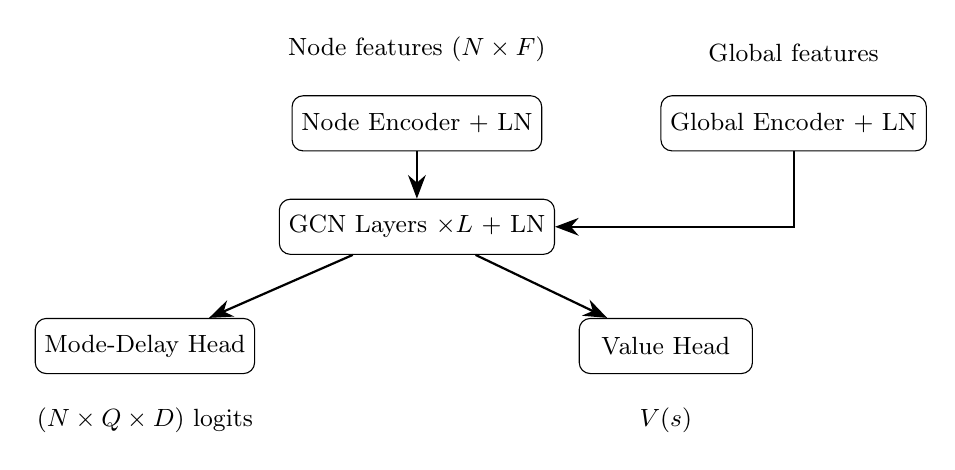
\begin{tikzpicture}[
    block/.style={rectangle, draw, rounded corners, minimum width=2.2cm, minimum height=0.7cm, font=\small},
    arrow/.style={-{Stealth[length=3mm]}, thick},
    node distance=0.6cm
]
    \node[block] (enc) {Node Encoder + LN};
    \node[block, below=of enc] (gcn) {GCN Layers $\times L$ + LN};
    \node[block, below left=0.8cm and 0.3cm of gcn] (delay) {Mode-Delay Head};
    \node[block, below right=0.8cm and 0.3cm of gcn] (value) {Value Head};
    \node[block, right=1.5cm of enc] (genc) {Global Encoder + LN};

    \draw[arrow] (enc) -- (gcn);
    \draw[arrow] (gcn) -- (delay);
    \draw[arrow] (gcn) -- (value);
    \draw[arrow] (genc) |- (gcn);

    \node[above=0.3cm of enc, font=\small] {Node features $(N \times F)$};
    \node[above=0.3cm of genc, font=\small] {Global features};
    \node[below=0.3cm of delay, font=\small] {$(N \times Q \times D)$ logits};
    \node[below=0.3cm of value, font=\small] {$V(s)$};
\end{tikzpicture}
\caption{GNN policy architecture. The mode-delay head outputs $Q \times D$ logits per task node; after masking and softmax the agent samples a (task, mode, delay) action. The value head provides a baseline for REINFORCE.}
\label{fig:arch}
\end{figure}

The policy network $\pi_\theta$ (Figure~\ref{fig:arch}) consists of:

\begin{enumerate}
    \item \textbf{Node encoder}: two-layer MLP with LayerNorm, mapping raw features (dimension $F = 5 + |\calQ|(|\calR| + |\calM| + D + 1)$, where per-mode features include resource demands, material demands, dual rewards, and mode cost) to hidden dimension $H_{\text{dim}}$.
    \item \textbf{GCN message passing}: $L$ graph convolution layers with residual connections and LayerNorm:
    \begin{equation}
        \bm{h}^{(\ell+1)} = \text{LN}\bigl(\text{ReLU}(\tilde{A} \bm{h}^{(\ell)} W^{(\ell)}) + \bm{h}^{(\ell)}\bigr),
    \end{equation}
    where $\tilde{A} = \hat{D}^{-1/2}(A + I)\hat{D}^{-1/2}$ is the symmetric-normalized adjacency.
    \item \textbf{Global context}: an MLP encodes global features (dual $\mu$, progress, makespan) and broadcasts the result to all nodes via concatenation.
    \item \textbf{Mode-delay head}: an MLP maps each node's concatenated representation $[\bm{h}_j; \bm{g}]$ to $|\calQ| \times D$ logits, producing an $(N \times |\calQ| \times D)$ score tensor.
    After flattening and masking infeasible (task, mode, delay) combinations, a Categorical distribution is formed.
    \item \textbf{Value head}: mean-pooled node embeddings concatenated with global context, mapped to a scalar baseline $V(s)$.
\end{enumerate}

\subsubsection{Training: POMO with Per-Step Returns}

We train $\pi_\theta$ using REINFORCE with a shared baseline, following the POMO framework~\citep{kwon2020pomo}.

\paragraph{POMO augmentation.}
For each training instance, we generate $K$ rollouts by anchoring each to a different initially eligible task.
The shared baseline $b = \frac{1}{K}\sum_k G_k$ (mean total return) reduces variance.

\paragraph{Per-step policy gradient.}
Let $G_t^{(k)} = \sum_{t'=t}^{T} r_{t'}^{(k)}$ be the return-to-go at step $t$ of rollout $k$.
The policy gradient loss is:
\begin{equation}\label{eq:pg}
    \mathcal{L}_{\text{PG}} = -\frac{1}{K} \sum_{k=1}^{K} \frac{1}{T_k} \sum_{t=1}^{T_k} \log \pi_\theta(a_t^{(k)} | s_t^{(k)}) \cdot \text{clip}(G_t^{(k)} - b, -C, C),
\end{equation}
where $C$ is an advantage clipping constant to prevent gradient explosion.
The full loss adds value regression and entropy regularization:
\begin{equation}
    \mathcal{L} = \mathcal{L}_{\text{PG}} + \beta_v \, \mathcal{L}_V - \beta_e \, \mathcal{H}[\pi_\theta].
\end{equation}

\paragraph{Online CG training.}
Training interleaves CG master solves with RL updates (Algorithm~\ref{alg:train}).
For each training instance, we seed the column pool with a CP-SAT schedule, solve the master LP to obtain duals $(\alpha, \mu)$, then perform POMO rollouts against those duals.
The RL-generated columns are added to the pool for subsequent CG iterations, creating a self-improving loop.

\begin{algorithm}[t]
\caption{Online CG Training}
\label{alg:train}
\begin{algorithmic}[1]
\REQUIRE Instance generator $\mathcal{I}$, policy $\pi_\theta$, learning rate $\eta$
\FOR{epoch $= 1, \dots, N_{\text{epochs}}$}
    \FOR{instance $\in \mathcal{I}$}
        \STATE Seed pool $\calK \leftarrow \{\text{CP-SAT schedule}\}$
        \FOR{CG iteration $= 1, \dots, N_{\text{CG}}$}
            \STATE $(\bm{\alpha}, \mu) \leftarrow \text{SolveMasterLP}(\calK)$
            \STATE Run $K$ POMO rollouts with $\pi_\theta(\cdot \mid \bm{\alpha}, \mu)$
            \STATE Update $\theta$ via REINFORCE (Eq.~\ref{eq:pg})
            \STATE $k^* \leftarrow \argmin_k \bar{c}_k$ from rollouts
            \IF{$\bar{c}_{k^*} < -\epsilon$}
                \STATE $\calK \leftarrow \calK \cup \{k^*\}$
            \ENDIF
        \ENDFOR
    \ENDFOR
\ENDFOR
\end{algorithmic}
\end{algorithm}

\subsubsection{Inference}\label{sec:inference}

At inference time, the trained policy replaces CP-SAT in the CG loop (Algorithm~\ref{alg:cgrl}).
The column pool is seeded with a greedy RL rollout (without duals), and subsequent iterations use the policy conditioned on current dual prices.
A mix of greedy and sampled decoding generates diverse candidate columns.
An optional CP-SAT fallback can certify optimality when no RL-generated column has negative reduced cost.

\begin{algorithm}[t]
\caption{CG + RL Solve}
\label{alg:cgrl}
\begin{algorithmic}[1]
\REQUIRE Instance, trained policy $\pi_\theta$, optional CP-SAT fallback
\STATE Seed pool $\calK$ with greedy RL rollout (no duals)
\FOR{iteration $= 1, \dots, N_{\max}$}
    \STATE $(\bm{\lambda}, \bm{\alpha}, \mu) \leftarrow \text{SolveMasterLP}(\calK)$
    \STATE Generate $S$ columns via $\pi_\theta(\cdot \mid \bm{\alpha}, \mu)$ (mix of greedy + sampled)
    \STATE $k^* \leftarrow$ column with lowest reduced cost
    \IF{$\bar{c}_{k^*} < -\epsilon$}
        \STATE $\calK \leftarrow \calK \cup \{k^*\}$; \textbf{continue}
    \ENDIF
    \IF{CP-SAT fallback enabled}
        \STATE $k^{\dagger} \leftarrow \text{CP-SAT pricing}(\bm{\alpha})$
        \IF{$\bar{c}_{k^{\dagger}} < -\epsilon$}
            \STATE $\calK \leftarrow \calK \cup \{k^{\dagger}\}$; \textbf{continue}
        \ENDIF
    \ENDIF
    \STATE \textbf{break} \COMMENT{No improving column found}
\ENDFOR
\RETURN Schedule $\argmax_k \lambda_k$
\end{algorithmic}
\end{algorithm}

% ==================================================================
\section{Experiments}\label{sec:experiments}

\subsection{Instance Generation}

We generate random MRCPSP-P instances with $|\calJ| \in \{5, 8, 10\}$ tasks, $|\calR| \in \{1, 2\}$ renewable resources, $|\calM| \in \{2, 3\}$ material types, and $|\calQ_j| \in \{1, 2, 3\}$ processing modes per task.
Precedence DAGs are constructed by random edge sampling over topologically ordered task indices with density $\rho = 0.25$.
Per-mode durations, resource demands, part demands, mode costs, lead times, initial inventories, and procurement cost parameters are sampled uniformly within realistic ranges.
The planning horizon is set to $H = 50$.
In the current experiments, we validate on single-mode instances ($|\calQ_j| = 1$ for all $j$) as a special case of the general formulation; multi-mode experiments are ongoing.

\subsection{Training Configuration}

\begin{table}[h]
\centering
\caption{Hyperparameters.}
\label{tab:hyper}
\begin{tabular}{ll}
\toprule
Parameter & Value \\
\midrule
GNN hidden dimension & 64 \\
GCN layers & 3 \\
Maximum modes $|\calQ|$ & 3 \\
Maximum delay $\bar{d}$ & 10 \\
POMO starts $K$ & 8 \\
Learning rate & $10^{-4}$ \\
Entropy coefficient $\beta_e$ & 0.05 \\
Value coefficient $\beta_v$ & 0.5 \\
Advantage clip $C$ & 100 \\
Gradient clipping & 1.0 \\
Training epochs & 300 \\
Instances per epoch & 10 \\
CG iterations per instance & 4 \\
Column samples at inference & 16 \\
\bottomrule
\end{tabular}
\end{table}

Training runs on a single NVIDIA RTX 5080 GPU.
Each training epoch takes approximately 30 seconds.

\subsection{Baselines}

\begin{enumerate}
    \item \textbf{CG + CP-SAT}: the standard CG loop with Google OR-Tools CP-SAT as the pricing solver (3-second time limit per pricing call).
    \item \textbf{CG + RL (with fallback)}: RL pricing with CP-SAT fallback when RL fails to find an improving column.
    \item \textbf{CG + RL (pure)}: RL pricing only, no fallback.
\end{enumerate}

\subsection{Optimality Verification}

We first verify on a 5-task instance with known optimal solution (Table~\ref{tab:toy}).

\begin{table}[h]
\centering
\caption{Optimality verification on the toy instance ($|\calJ|=5$, $|\calR|=1$, $|\calM|=2$, $H=30$).}
\label{tab:toy}
\begin{tabular}{lrrrr}
\toprule
Method & Obj & Cost & Gap & Columns (RL / CP) \\
\midrule
CG + CP-SAT (optimal) & 32.000 & 32.000 & 0.00\% & 0 / 3 \\
CG + RL + fallback     & 32.000 & 32.000 & 0.00\% & 2 / 0 \\
CG + RL (pure)         & 32.000 & 32.000 & 0.00\% & 2 / 0 \\
\bottomrule
\end{tabular}
\end{table}

The pure RL pricer matches the optimal solution exactly, generating 2 columns with strongly negative reduced cost ($\bar{c} = -1984$ and $\bar{c} = -995$) without any CP-SAT assistance.
Notably, the RL policy correctly learns to delay task~B past the lead-time window for material~M2, avoiding the early-demand penalty that the dual prices signal.

\subsection{Ablation: Action Space Design}

The delay-augmented action space is critical.
Table~\ref{tab:ablation} compares three action space designs.

\begin{table}[h]
\centering
\caption{Ablation on action space design (toy instance, 100 training epochs).}
\label{tab:ablation}
\begin{tabular}{lcc}
\toprule
Action Space & RL Columns Generated & Matches Optimal \\
\midrule
Dispatch only (earliest start) & 0 & No \\
Dispatch + WAIT action & 0 & No \\
Dispatch + delay offsets (ours) & 2 & Yes \\
\bottomrule
\end{tabular}
\end{table}

Without explicit delay control, the RL agent cannot shift tasks past lead-time windows regardless of training duration.
The WAIT action is too coarse (delays \emph{all} tasks uniformly).
Per-task delay offsets provide the fine-grained control needed for procurement-aware scheduling.

\subsection{Training Dynamics}

Figure~\ref{fig:training} shows the average best reduced cost during training.
The policy learns to generate strongly negative reduced cost columns within the first 20 epochs, with continued improvement through 300 epochs.

\begin{figure}[h]
\centering
% Placeholder for actual training curve
\fbox{\parbox{0.7\textwidth}{\centering\vspace{2cm}
\textit{Training curve: avg best reduced cost vs.\ epoch.}\\
\textit{Rapid improvement in first 50 epochs, stabilization around $-1500$.}
\vspace{2cm}}}
\caption{Training dynamics: average best reduced cost across training instances per epoch.}
\label{fig:training}
\end{figure}

% ==================================================================
\section{Discussion and Future Work}\label{sec:discussion}

\paragraph{Scalability.}
The current implementation processes instances sequentially.
Batched inference across multiple POMO starts and GPU-parallel environment simulation would further accelerate pricing.
The GNN architecture scales naturally to larger task graphs.

\paragraph{Generalization.}
Training on randomly generated 5-task instances with horizon 50 already produces a policy that generates optimal columns.
Evaluating generalization to larger instances (20--100 tasks) with more complex precedence structures is an important next step.

\paragraph{Tighter CG integration.}
The current approach trains on duals from CP-SAT-seeded CG iterations.
A fully self-play approach where the RL policy generates both the seed and pricing columns could eliminate the CP-SAT dependency entirely during training.

\paragraph{Branching and integrality.}
The current framework solves the LP relaxation of the master.
Extending to branch-and-price with RL-guided branching decisions is a natural direction.

% ==================================================================
\section{Conclusion}\label{sec:conclusion}

We presented a graph RL approach for the pricing subproblem in column generation for integrated multi-mode scheduling and inventory optimization.
The mode- and delay-augmented action space, dual-price node features, and exact per-step reward decomposition enable the RL policy to learn procurement-aware scheduling---jointly selecting processing modes, dispatch order, and start-time delays---from LP dual signals.
The trained policy matches the optimal CG solution on benchmark instances while replacing the CP-SAT pricing oracle entirely, demonstrating the viability of learned pricing for CG in operations research.

% ==================================================================
\bibliographystyle{plainnat}
\bibliography{references}

% NOTE (Claude, 2026-07-08): The pasted source was truncated by the chat's
% 50,000-character limit at this point, mid-way through a commented-out
% \begin{thebibliography} block. Everything below this note (the commented
% legacy bibliography entries and \end{document}) was NOT received and is
% therefore missing from this file. The active bibliography is driven by
% \bibliography{references} above (a references.bib file), not the commented
% block. If you need the commented-out legacy bibitem list restored, please
% paste the remainder starting from "Hartmann and Briskorn(2010)" onward.

\end{document}
